\subsection{Software Implementation}
Software is one of the essentials of the product, it is also one of the challenges for the business to exist. Since a business plan describes the fundamentals of the company and how it is going to make money, it is a critical section to describe the product, which will be done during this section. When there is a need of developing a software, the usual way would be to collect requirements from stakeholders. Currently the group is the only known stakeholder and therefore it is hard to create the usual procedure for the development. This would be a acquiring of requirements, create use cases, design a class diagram and keep it developed during the process. 

The development process is one of the key activities during the start up of the company. Therefore it is important to have focus of this specific process and making the choice of the right process. When in need of rapid development activities within the Scrum process would be attractive for the group, because it would implement the daily meeting which is used for sharing of problems and ideas for solving them. This requires an expert knowledge to become a useful process, which the group is eligible of.
\thomas{Not a big fan of the sudden clearpage - We end up with a humongous pile of random whitespace. Whitespace is to be avoided at all cost}
\clearpage
\paragraph*{Structure of the Software System}
Figure \ref{ClassDiagram} shows the current state of the architecture of the software system. The system is not yet complete and will grow during the development process. The modifications are hard to predict at this very moment, but this displays the main functions of the system and what focus areas there are within the development. 
\begin{figure}[h!]
\centering
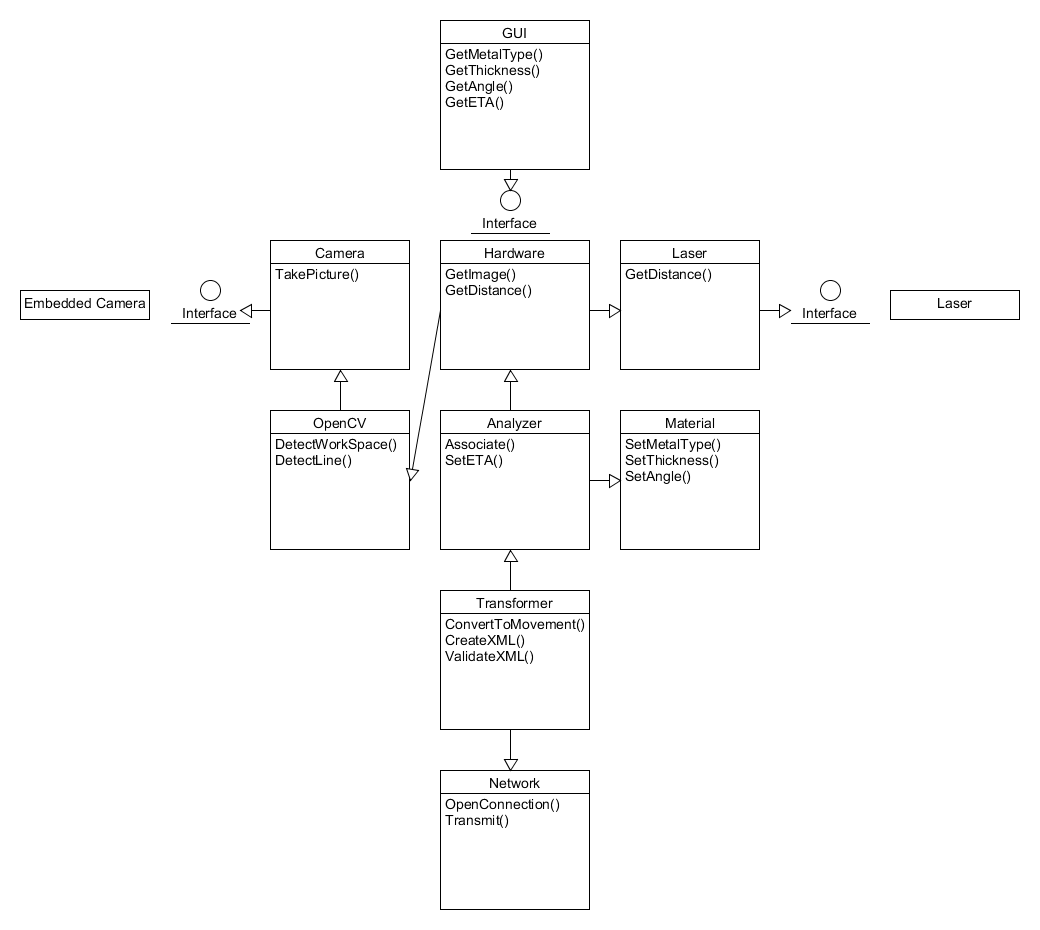
\includegraphics[width=0.7\textwidth]{graphics/ClassDiagram}
\caption{A simple class diagram for the prototype software system}
\label{ClassDiagram}
\end{figure}
The system is going to consist of multiple hardware parts, these parts will require interfaces for communication. This communication is going to happen not only between hardware, but also internally between different parts of the software.
In this section, these different interfaces will be described. 

\paragraph*{Hardware Interfaces}~\\
Hardware, in the form of sensors, is a major part of the product. These will require interfaces to communicate with the software system. The default software for these hardware parts does not necessarily output comparable data. The usual way to approach this issue is to implement adapter patterns, which includes a facade pattern. Two hardware interfaces are used in the system:

\begin{itemize}

\item Adapter pattern for the Laser Scanner output software
\item Network Interface between Add-On and a potential robot

\end{itemize}

The camera and the laser scanner will most likely come from different manufacturers, therefore there is no guarantee for compatibility of the included software. This is where an adapter pattern becomes useful within the system.

The network interface will have to fit any standards that exist for robotic interfaces. Additionally the interface is very dependant on the specific partner's software and their choice of robotic interfaces.
\paragraph*{Software Interfaces}~\\
Software interfaces are often used when it comes to the facade of a system. This helps making the objects unknown to other objects in the system. The purpose is to make a system with low coupling and high cohesion. Interfaces are also common to use when you have several objects or classes which need the same method, so to lower the amount of 'copy + paste' code, you should implement interfaces instead. It is hard to identify methods that should be reinvented within the current prototype class diagram, which is why this section will not cover them. That is why the class diagrams will be updated during the development process of the software. There are two different software interfaces used in the system:

\begin{itemize}

\item Facade pattern for the embedded camera
\item Facade pattern between user interface and logic layer

\end{itemize}

\paragraph*{User Interfaces}~\\
The main issue when designing a user interface is to keep it user friendly, however, it is still important that the requirements set by the stakeholders are taken into careful consideration. During the design process these requirements should be updated frequently to avoid any misunderstandings.

The add-on will come with a tablet which will be the platform for the user interface. Different functionalities are provided by this interface: 

\begin{itemize}

\item Selection of material to weld 
\item Define thickness of the object
\item Welding angle of the robot
\item Overview of different data, like ETA of the current welding, range of the laser scanner

\end{itemize}

This enables the end user to modify the welding process in a few steps. Importance of user friendliness is immense, since the time spent on modifying the process has to be compared to the time the user could spend somewhere else.

\subsubsection{Specific requirements}
Requirements are fundamental to specify the tasks to solve when creating a software system. Requirements can be divided into categories as seen here:

\textbf{Functional Requirements:}
\begin{itemize}

\item The system should be able to communicate with the specified hardware
\item The system should be able to communicate with any welding robot of potential future partners
\item The system should be able to take pictures with an embedded camera 
\item The system should be able to detect a line within the workspace of each picture provided by the embedded camera, by using OpenCV
\item The system should be able to create three dimensional coordinates based on inputs from a range scanner and a camera
\item The system should be able to convert movement-coordinates for a specific robot

\end{itemize}

\textbf{Non-functional Requirements:}

\begin{itemize}

\item The system should be able to create a path for the robot within one tenth of the time it takes to pickup the coordinates.
\item The precision of the laser should be $\pm$0.05 cm

\end{itemize}

\paragraph*{Functions}

The system can be divided into three major functions, which handles the process of detecting the place to weld, associate x, y and z coordinates and convert them into the movement program of a robot.

These actions can be divided into the following functions:

\begin{itemize}

\item \textbf{DetectLine:} Using functionality from the OpenCV library, this function is to detect the workspace area, by detecting the color marked by a worker, then detecting the line within.
\item \textbf{Associate:}This class has the task of gathering the two different data (camera coordinations and laser depth coordinations).
\item \textbf{ConvertToMovement:} The final coordinates generated from the Associate class is being converted to an input which a robot can use. 

\end{itemize}

\subparagraph*{System attributes}~\\
System attributes describes the qualities of a system in short terms. Primary qualities of the system is going to be:

\begin{itemize}

\item Reliability
\item Precision
\item Maintainability
\item Adaptability
. 
\end{itemize}
These are the attributes needed for a system to be able to adapt to any robot welding system, while maintaining its reliability and precision. These keywords are to be kept in mind when developing the system at all times.

\subparagraph*{Dependencies}~\\
Using libraries can create dependencies within the system, mainly when a used library is dependant on other libraries. This can cause multiple version dependencies and cause a chain of them. In this project, the OpenCV library will be in focus when extracting data of the line that the robot has to weld. The term 'Dependency Hell' is used to describe the situation explained above. Developers of the project have to be aware of this problem. It is possible to solve it by using package managers that can solve dependencies automatically by updating libraries to the correct versions. 

\subparagraph*{Database}~\\
A database to log every entry is favourable for the end customer, but it is not a part of the add-on and therefore not a part of the development process.
\thomas{If it is favourable for the end user to HAVE a database but we decide not to provide it, we better come up with a good reason for not providing it}

\subsubsection{Design decisions}
Basically the system is set to follow the 3 layer structure. But as the system evolves it can be hard to predict whether this is going to change or not. 

A factor which is common in the industry, is the request for real time actions within a network. Real time is when a system can deliver every time it is needed. Real time is very network dependant because of the deadlines within an automated production. 
Real time is not requested in our system, since a worker handles the robot and leaves it for its time to work. This mean that no special BUS networks are needed within the system and that a TCP protocol Ethernet network is a viable option. TCP allows packet loss on a network with the consequence of retransmission.

In general this mean that the end customers will not have to implement an expensive network between our add-on and the robot. 

\subsubsection{Life cycle}

When the product has been developed and released it is far from complete, this is the reason for maintenance and repeating the working process of optimization and development. If the product is not updated, competitors and new ideas on the market will quickly surpass our product. Therefore it is important to repeat the actions described in the life cycle below:
\clearpage

\begin{figure}[ht]
\centering
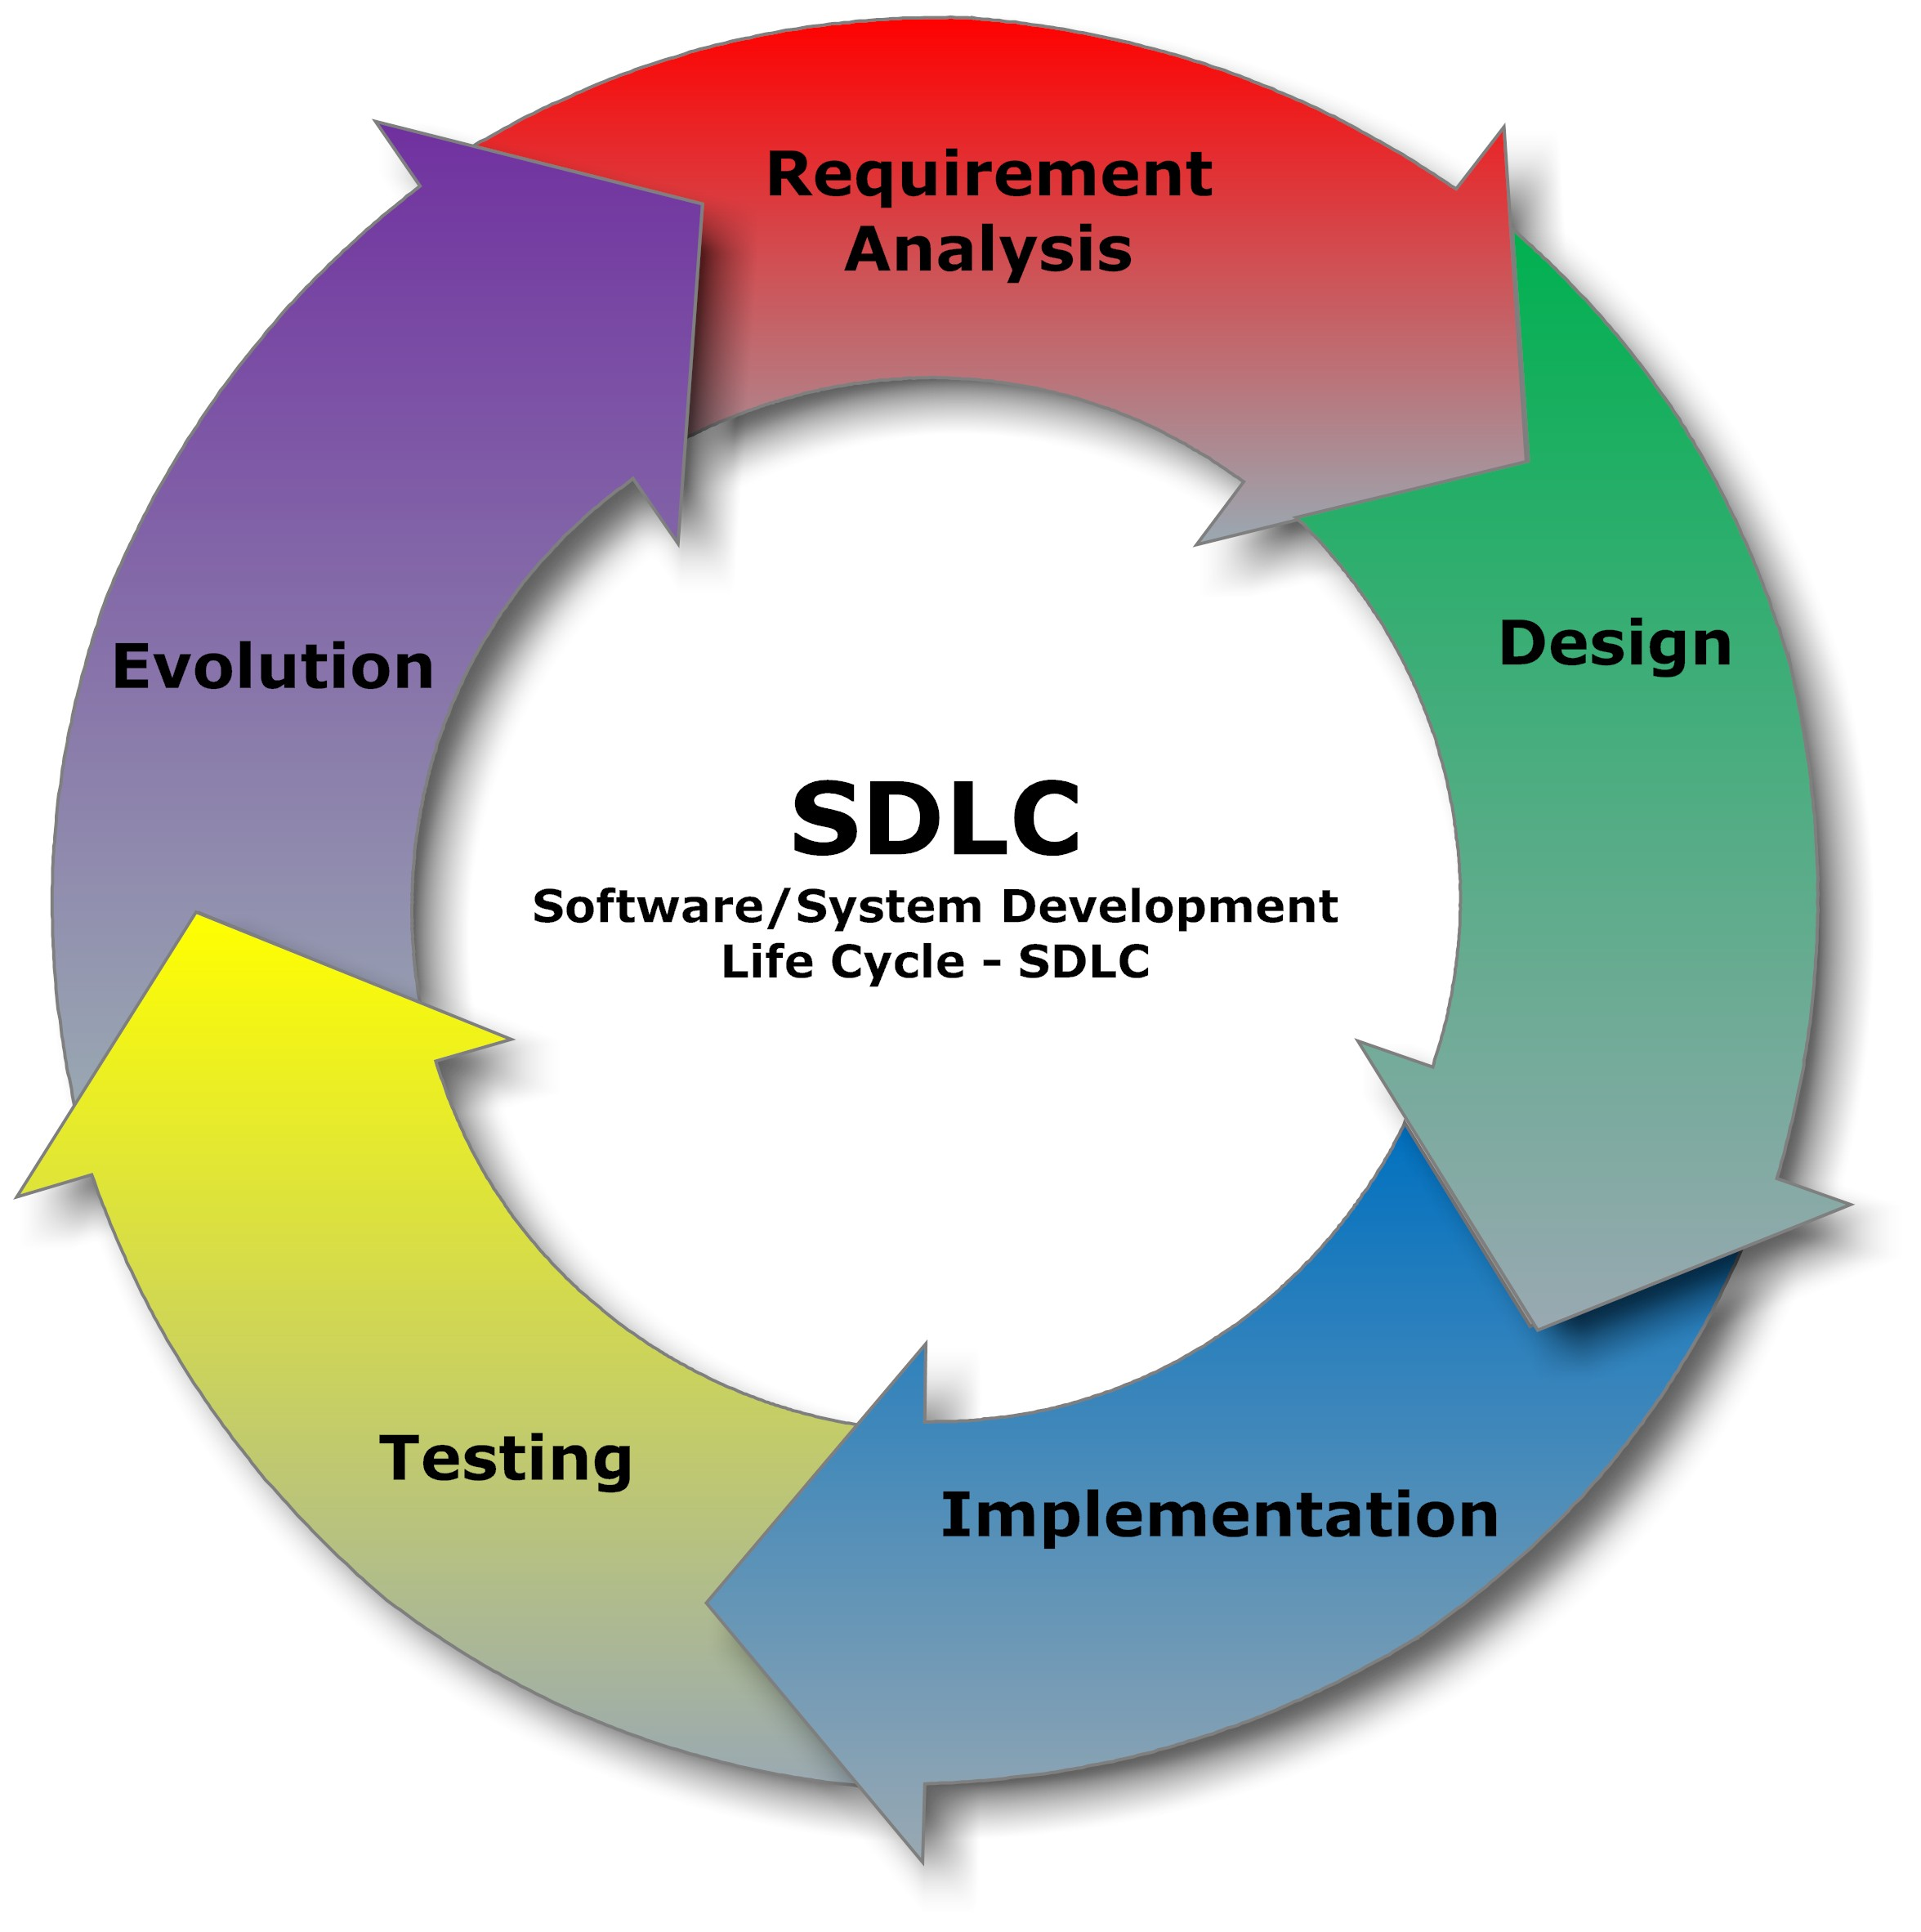
\includegraphics[width=0.5\textwidth]{graphics/Software_Development_Life_Cycle}
\caption{The life cycle describes the process of establishing and maintaining a system}
\label{SDLC}
\end{figure}
This process is not very detailed, because it is up to the developers and manage to choose a specific development process or a combination of them. But the actual purpose of the model is to go through the primary phases of software development in a correct order. With a start at gathering requirements ending in an evolution of the software. Each iteration should result in a new and patched version of the software. The actual model shows a waterfall model, which have major areas to focus on at a time. By following this model you can avoid doing dependant activities too early in the process.
